\chapter{Rocket Analysis}\label{chap:RockAnalyis}

\todo{Appendix refference not working, find a way to include path i guess.}
		A rocket presents a large number of similarities with an inverted pendulum in terms of modeling and control as it will be demonstrated in this chapter. It also adds one degree of freedom compared to the inverted pendulum, since it can be controlled in two horizontal directions. A model of the rocket is made to be able to compare the two systems' dynamics.
		\\
		Two different parameters can be controlled in the rocket: the angle of its body compared to vertical and its position.
		The purpose is to minimize the angle and to keep the initial position, but not the initial altitude.
		
%		The angle to position was taken out. if put back, change the intro
		
		\section{Modeling of the angle}
		\begin{figure}[htbp]
			\centering
			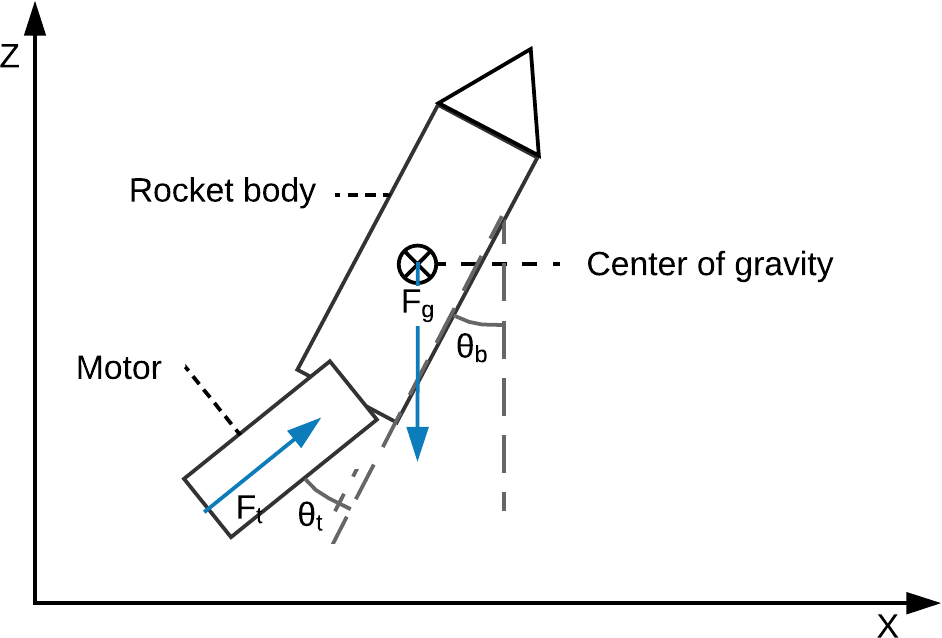
\includegraphics[width=0.7\textwidth]{figures/modeling/Rocket/rocket_angle_diagram.png}
			\caption{Simplified sum of forces on the rocket.}
			\label{fig:angle_diagram}
		\end{figure}
		
		This section will focus on the forces acting perpendicularly to the rocket body, thus creating torques.
		The resulting transfer function will take $\theta_t$, the thruster angle compared to the body, as an input and $\theta_b$, the body angle compared to vertical as an output.
		
		The thruster force $F_t$ will be considered as constant. See the rocket motor test experiment for details: \autoref{ThrusterTest}. $F_g$ is the gravity force on the rocket's center of gravity. The force of drag is neglected due to the low-speed conditions of the tests, and the absence of air in most real-life scenarios.


		
%		Let's call $l_{Cg}$ the distance between the center of gravity and the end of the thruster.
		Using Newton's second law the following equation can be derived.

		\begin{equation}
			I_r \cdot \ddot{\theta_b}=\tau_t \addunit{\newton$\cdot$\meter} \label{eq:rocket_angle_1}
		\end{equation}
		\startexplain
			\explain{$I_r$ is the inertia of the rocket}{\si{\kilo\gram$\cdot$\meter^2}}
			\explain{$\ddot{\theta_b}$ is the angular acceleration of the rocket body}{\si{\second^{-2}}}
			\explain{$\tau_t$ is the torque created by the thruster on the rocket}{$\si{\kilo\gram \cdot\meter^{2}\cdot\sec^{-2}}$}
		\stopexplain
		
%		$\tau_t$ can be expressed as:
%		
%		\begin{equation}
%		\tau_t=f_t \cdot \theta_t \cdot l_{Cg} \addunit{\newton$\cdot$\meter} \label{eq:rocket_angle_2}
%		\end{equation}
%		\startexplain
%		\explain{$\theta_t$ is the angle of the truster compared to the rocket body}{1}
%		\explain{$f_t$ is the thrust force}{\si{\newton}}
%		\stopexplain
		
		By going to the Laplace domain and grouping elements the following transfer function is obtained:
%		
%		\begin{equation}
%		\frac{\theta_b}{\theta_t} = \frac{f_t \cdot l_{Cg} \cdot \frac{1}{I_r}}{s^2}
%		\label{eq:rocket_angle_model_tf_1}
%		\end{equation}
		
		Calculating $I_r$ assuming that all the mass is concentrated at the electronics/battery stage of the rocket. $70\%$ of the weight is in fact concentrated on this part (rocket is about $300$ grams and the electronics stage is around $0210$ grams). The rocket is rotating around its center of gravity.
		
		\begin{equation}
		I_r=m_{Es} \cdot l_{Es}^2 \label{eq:rocket_angle_3}
		\end{equation}
		\startexplain
		\explain{$m_{Es}$ is the mass of the electronics stage}{\si{\kilo\gram}}
		\explain{$l_{Es}$ is the distance from the electronics stage to the center of gravity}{\si{\meter}}
		\stopexplain
		
		The torque $\tau_t$ can be expressed as:
		\begin{equation}
		\tau_t = F_t \cdot sin(\theta_t) \cdot l_{Cg} \addunit{\newton$\cdot$\meter} \label{eq:tau_t}
		\end{equation}
		\startexplain
		\explain{$F_t$ is the thruster force}{\si{\newton}}
		\explain{$\theta_t$ is the angle of the thruster compared to the body's longitudinal axis}{1}
		\explain{$l_{Cg}$ is the distance from the thruster end to the center of gravity}{m}
		\explain{$\tau_t$ is the torque created by the thruster on the rocket}{\si{\newton \meter}}
		\stopexplain
		
		The small angle approcimation is used on $\tau_t$:
		\begin{equation}
		\tau_t = F_t \cdot \theta_t \cdot l_{Cg} \addunit{\newton$\cdot$\meter} \label{eq:tau_t_lin}
		\end{equation}
		
		The transfer function becomes:
		\begin{equation}
		H=\frac{\theta_b}{\theta_t} = \frac{F_t \cdot l_{Cg} \cdot \frac{1}{m_{Es} \cdot l_{Es}^2}}{s^2}
		\label{eq:rocket_angle_model_tf_2}
		\end{equation}
		
		The servomotors also present a transfer function to be taken into consideration. The transfer function is obtained in \autoref{eq:servo_models}. It is a first order system. The time constant of the servomotors is determined in \autoref{ssc:Servomotors}.
		
		\begin{equation}
		\frac{\theta_{out}}{\theta_{in}}=\frac{1}{\tau s + 1}  \label{eq:servo_model}
		\end{equation}
		\startexplain
		\explain{$\theta_{in}$ is the angle sent to the servo by the controller}{1}
		\explain{$\theta_{out}$ is the angle outputed by the servo}{1}
		\stopexplain
		
\section{Comparison of the Inverted Pendulum and Rocket Models}\label{sec:ModelComp}

From \autoref{chap:IPAnalysis} and \autoref{chap:RockAnalyis} it is found, that the models are slightly different. First of all, opposite angles were chosen in the beginning of the modeling process. Moreover, the inverted pendulum is fixed to the gears and motor, while the rocket is floating in the air, and thus canceling the gravity. The inverted pendulum has two more zeros in 0 and two real poles equidistant from zero, whereas the rocket has two poles in 0. The difference in poles is due to the absence of gravity into the rocket modeling, while the difference in zeros might be due to the fact that the arm is rigidly attached compared to the thruster.

Due to this difference a different controller needs to be designed for each model.
		
%		
%		\section{Modeling of the horizontal position}
%
%		To finish:
%		different diagram of the rocket, similar to figure 6.1 .
%
%		This part will focus on the forces acting on the rocket in the horizontal axis.
%		The resulting transfer function will take $\theta_t$, the thruster angle compared to the body, as an input and $x$, the horizontal position of the rocket as an output.
%
%		The thruster force $F_t$ will be considered as constant. See the rocket motor test experiment for details \todo[inline, author=Paperboy]{Add vref for SRB test experiment}. The force of drag is neglected due to the low-speed conditions of the tests, and the absence of air in most real-life scenarios. The force of lift is neglected as well.
%
%		Let's call $\theta_t$ the angle between the thruster and the vertical axis.
%		Using Newton's second law the following equation can be derived.
%
%		\begin{equation}
%			M_r \cdot \ddot{x} = F_t \cdot \sin(\theta_r)
%			\addunit{\newton}		 
%			\label{eq:rocket_position_1}
%		\end{equation}
%		\startexplain
%		\explain{$M_r$ is the mass of the rocket}{\si{\kilo\gram}}
%		\explain{$\ddot{x}$ is the acceleration of the rocket on the horizontal axis}{\si{\meter\per\second^{-2}}}
%		\stopexplain
%
%		$\theta_r$ can be expressed as:
%
%		\begin{align}
%			\theta_r = \theta_b + \theta_t 
%			\theta_b = \theta_t \cdot C \label{eq:rocket_total_angle}
%		\end{align}
%		\startexplain
%		\explain{$C$ is the relation found in \ref{rocket_angle_model_tf_2}{1}
%		\stopexplain
%	
%		By going to the Laplace domain and grouping elements the following transfer function is obtained:
%	
%		\begin{align}
%			\frac{X}{\theta_t} = \frac{F_t \cdot (1 + C) }{M \cdot s^2}
%			\addunit{\meter} 
%			\frac{X}{\theta_t} = \frac{s^2 \cdot (M_r \cdot l_{Es}^2 \cdot F_t) + F_t^2 \cdot 	l_{Cg}}{s^4 \cdot M_r^2 \cdot l_{Es}^2}
%			\label{eq:rocket_positon_tf_1}
%		\end{align}
%	
%	
%	\todo[inline, author=Paperboy]{Sort out the "relevent" commented text}
	%				\section{Inverted pendulum and rocket}
	%			The goal of this section is to demonstrate the similarities between the inverted pendulum and the rocket stabilization processes, and to define a mathematical model and control loop of the behavior of the angle of the rocket body and the angle of the thruster.
	%			
	%			The purpose of the system is to guarantee a stable flight to the rocket.
	%			The modeling of the flight of a rocket can be divided into two equations: velocity and rotation. In this project, the desired trajectory of the rocket flight is considered to be on the zenith axis. This results in a vertical flight, with then a velocity on the same axis as the trajectory.The rocket's rotation is a circular motion on the bottom-to-nose axis. This create a centripetal force.
	%			
	%			The displacement angle (gimbal angle) is the difference between the actual flight direction, or bottom-to-nose axis, and the zenith axis. Gimbaled thrust are controllable thrusters used to create a torque and reduce the gimbal angle. 
	%			
	%			In an inverted pendulum, the objective is to keep the stick in horizontal position. The angle difference between the horizontal and the actual axis of the stick is measured in order to then create a compensation torque with the arm. The arm has the same task as the gimbaled thruster, and the horizontal axis is equivalent to the zenith axis.
	%			
	%			At the desired initial position of the inverted pendulum, the acceleration of the arm is negligible. This implies that the arm only produces a force on the axis going through the center of gravity of the arm and parallel to the lenght of the arm. This is equivalent to the rocket process where the thruster applies a force on the axis going through the center of gravity of the arm and parallel to the lenght of the thruster. 
	%			
	%			 Sketch of rocket + IP at initial position
	%			
	%			Therefore the rocket and the inverted pendulum processes are equivalent for a small displacement angle range. The inverted pendulum is then studied in this project as a first approach to the understanding of rocket in-flight stabilization process.
	%			
	%			The control loop of the rocket system is described in figure ...
	%			
	%			Figure of closed loop model of rocket
	%			
	%			The input of the closed loop is the gimbal angle (angle difference between actual flight direction and zenith axis). The output is the new gimbal angle. In the inverted pendulum, the input and output are also the angle differences, between the horizontal and the actual axis of the stick. 
	%			
	%			By admiting that the inverted pendulum and the rocket processes are similar the equations found in Section 5.2 Modelling of the Arm and Stick can be applied to the rocket, with the rocket body as the stick and the gimbaled thruster as the arm. However the gravity center of the rocket body is not located in its center. Therefore $l_{a}$ and $\frac{l_{s}}{2}$ become respectively $l_{t}$, for the thruster, and $l_{bg}$, for the lenght from the bottom of the rocket body to its center of mass. The equations describing the forces, with $a$ for arm and $s$ for stick respectively replaced by $t$ for thruster and $b$ for rocket body, are:
	%			
	%			Transfer function as in part "modeling of stick".
	
	%		\section{Modeling of the rocket body and stick}
	%			
	%		The purpose of this section is to have a mathematical model for the different forces applied on the rocket in flight. 
	%		
	%		In this project, only the upward movement will be studied, as the downward movement does not need control due to a parachute controlling the rocket's fall. The trajectory of the rocket is on the zenith axis, or y axis.   Moreover the upward rocket movement will be at low speed. This implies the impact of the lift on the rocket is negligible. The sum of the forces applied on a rocket in flight can then be described by equation \vref{eq:F_total}:
	%		
	%		\begin{equation}
	%		F_{total} = m*a = F_{thrust} + F_{drag} - F_{gravity} \addunit{\newton} \label{eq:F_{total}}
	%		\end{equation}
	%		\startexplain
	%		\explain{$F_{total}$ is the sum of all force}{\si{\newton}}
	%		\explain{$F_{thrust}$ is the force created by the gimbaled thruster}{\si{\newton}}
	%		\explain{$F_{drag}$ is the drag force on the rocket}{\si{\newton}}
	%		\explain{$F_{gravity}$ is the gravity applied on the rocket}{\si{\newton}}
	%		\stopexplain
	%		
	%		The drag force can be expressed by equation \vref{eq:F_drag}:
	%		\begin{equation}
	%		F_{drag} = \frac{1}{2} \cdot C_{d} \cdot \rho \cdot A \cdot v^2 \si{\newton} \label{eq:F_{drag}}
	%		\end{equation}
	%		\startexplain
	%		\explain{$C_{d}$ is the coefficient of drag}{\si{1}}
	%		\explain{$\rho$ is the air density}{\si{\kilo\gram\per\meter\cubed}}
	%		\explain{$A$ is the cross sectionnal area of the rocket}{\si{\meter\squared}}
	%		\explain{$v$ is the velocity of the rocket}{\si{\meter\per\second}}
	%		\stopexplain
	%			
	%		The coefficient of drag and the cross sectionnal area vary depending on the shape of the rocket. Altitude and humidity in the air can impact the air density. Parasit drag can appear due to the surface material or pressure drag.
	%		
	%		The gravity force equation is \vref{eq:F_{gravity}}:
	%		\begin{equation}
	%		F_{gravity} = m \cdot g \addunit{\newton} \label{eq:F_{gravity}}
	%		\end{equation}
	%		\startexplain
	%		\explain{$m$ is the mass of the rocket}{\si{\kilo\gram}}
	%		\explain{$g$ is the gravitational acceleration}{\si{\meter\per\second\squared}}
	%		\stopexplain
	%			
	%		
	%		The thrust force is \vref{eq:F_{thrust}}:
	%		\begin{equation}
	%		F_{thrust} = v_{e} \cdot \ddot{m} + A (P_{e} -P_{0}) \addunit{\newton} \label{eq:F_{thrust}}
	%		\end{equation}
	%		\startexplain
	%		\explain{$v_{e}$ is the velocity of the gimbaled thruster}{\si{\meter\per\second}}
	%		\explain{$\ddot{m}$ is the mass flow rate}{\si{\kilo\gram\per\second}}
	%		\explain{$A$ is the nozzle exit area}{\si{\meter\squared}}
	%		\explain{$P_{e}$ is the pressure of the nozzle exit}{\si{\kilo\gram\per\meter\per\second\squared}}
	%		\explain{$P_{0}$ is the free stream pressure}{\si{\kilo\gram\per\meter\per\second\squared}}
	%		\stopexplain
	%		
	%		
	%		The thruster pression and velocity is divided into two equation, respectively ahead and behind the propeller nozzle: $P_{o}$ \vref{eq:P_{o}} and $P_{e}$ \vref{eq:P_{e}}.
	%		
	%		\begin{equation}
	%		P_{0} = p_{0} + 0.5 \cdot \rho \cdot(v_{o})^2 \addunit{\kilo\gram\per\meter\per\second\squared} \label{eq:P_{o}}
	%		\end{equation}
	%		\startexplain
	%		\explain{$p_{o}$ is the static pressure}{\si{\kilo\gram\per\meter\per\second\squared}}
	%		\explain{$v_{o}$ is the velocity of the rocket}{\si{\meter\per\second}}
	%		\stopexplain
	%		
	%		\begin{equation}
	%		P_{e} = p_{o} + 0.5 \cdot \rho \cdot(v_{e})^2 \si{\kilo\gram\per\meter\per\second\squared} \label{eq:P_{e}}
	%		\end{equation}
	%		\startexplain
	%		\explain{$v_{e}$ is the exit velocity of the gimbaled thruster}{\si{\meter\per\second}}
	%		\stopexplain
	%		
	%		Therefore, there is three different cases of truster pression:
	%		\begin{equation}
	%		P_{e} = P_{a} \notag
	%		 P_{e} > P_{a} \notag
	%		 P_{e} < P_{a} \notag
	%		\end{equation}
	%		 \todo[inline, author=Geoff]{copy paste equation syntaxe from above sections to have multiple equations}
	%		 insert sketch of the different cases
	%		 
	%		 \section{Linearization}
	%		
	%		\startexplain
	%		\explain{$F_x$ is the force in the x direction}{\si{\newton}}
	%		\explain{$F_y$ is the force in the y direction}{\si{\newton}}
	%		\explain{$x_b$ is the position of the center of gravity of the rocket in the x direction}{\si{\meter}}
	%		\explain{$y_b$ is the position of the center of gravity of the rocket in the y direction}{\si{\meter}}
	%		\explain{$l_t$ is the length of the thruster}{\si{\meter}}
	%		\explain{$C_g$ is the length between the gimbal and the center of gravity of the rocket}{\si{\meter}}
	%		\explain{$\theta_t$ is the angle from the thruster to the y-axis}{\si{\radian}}
	%		\explain{$\theta_b$ is the angle from the rocket body to the y-axis}{\si{\radian}}
	%		\stopexplain
	%		All forces, constants and variables that relates to the thruster and rocket body are denoted by a subscripted $t$ and $b$ respectively. 
	%		
	%		The behaviour of the rocket can be fully described by three movements; two translatory and one rotary. It can move in the x and y direction and rotate around its own axis.
	%		
	%		%To find the relation between the angles, the free body diagram of the joint of the arm and stick is made on \autoref{fig:freebodystick}.
	%		%\begin{figure}[htbp]
	%		%\centering
	%		%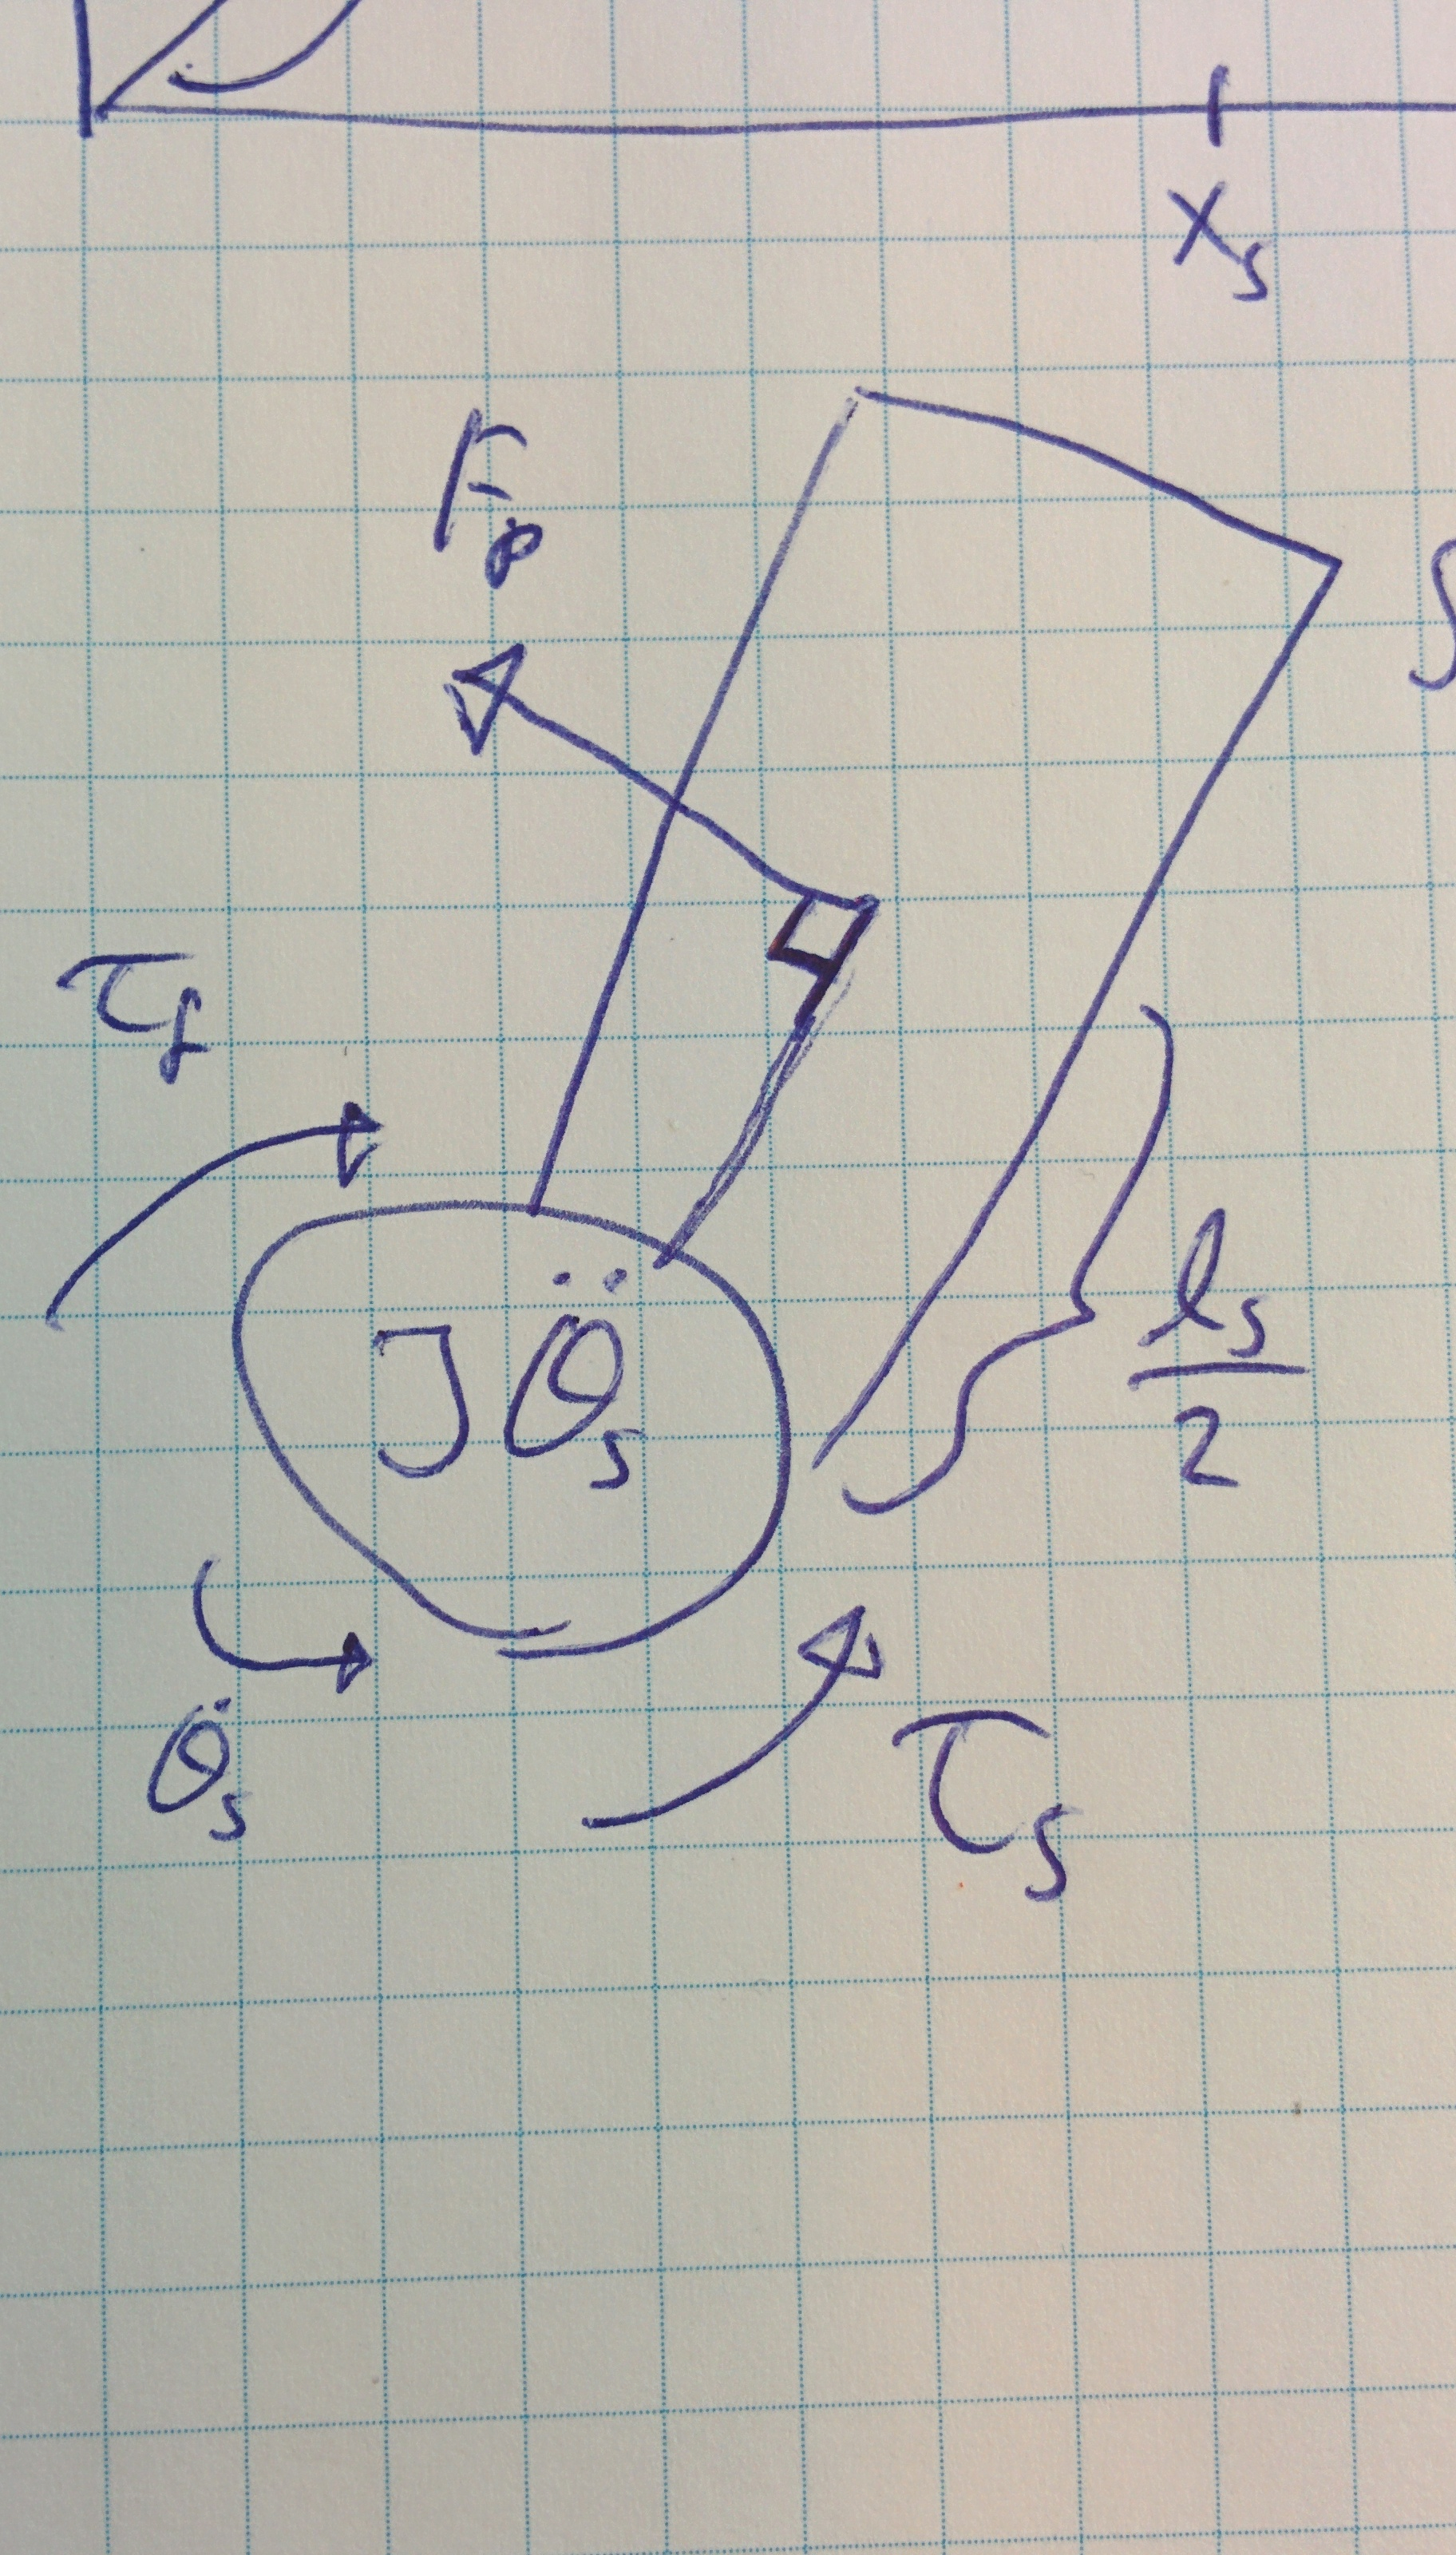
\includegraphics[width=0.25\textwidth]{FreeBodyPendulum}
	%		%\caption{Free body diagram of the joint that connects the arm and the stick.}
	%		%\label{fig:freebodystick}
	%		%\end{figure}
	%		%\todo[inline, author=Jacob]{Make pretty graph}
	%		%
	%		%The moment of inertia for the joint is described by \autoref{eq:Jrthetas}.
	%		%\begin{subequations}
	%		%\begin{flalign}
	%		%& J_r\ddot{\theta}_s=\tau_s-\tau_f  \label{eq:Jrthetas} \\
	%		%& \tau_s =F_p\frac{l_s}{2} \\
	%		%& \tau_f =b_{as}\dot{\theta}_{as} 
	%		%\end{flalign}
	%		%\end{subequations}
	%		%\startexplain
	%		%	\explain{$J_r$ is the moment of inertia for the stick}{\si{\kg\square\meter}}
	%		%	\explain{$\ddot{\theta}_s$ is the angular acceleration of the stick}{\si{\radian\per\square\second}}
	%		%	\explain{$\tau_s$ is the torque induced by the rotation of the stick}{\si{\newton\meter}}
	%		%	\explain{$\tau_f$ is the torque of the friction acting on the stick}{\si{\newton\meter}}
	%		%	\explain{$F_p$ is the force perpendicular to the stick at the center of mass}{\si{\newton}}
	%		%	\explain{$b_{as}$ is the viscous friction coefficient between the arm and the stick}{\si{\newton\meter\second}}
	%		%	\explain{$\dot{\theta}_{as}$ is the difference in angular velocity between the arm and the stick ($\dot{\theta}_s-\dot{\theta}_a$)}{\si{\radian\per\second}}
	%		%\stopexplain
	%		%
	%		%The friction is calculated from the difference in angular velocity as the stick could be perfectly upright while the arm moves causing the joint to turn. The angle of the arm is not considered as producing a torque acting on the joint but as part of the force on the stick, $F_p$.
	%		
	%		The forces acting on the rocket in the x and y directions are found by \vref{eq:FxFyRocket} using Newton's 2nd law of motion. Unlike in the inverted pendulum, there is no reaction to gravity from the arm, thus gravity does not produce any torque.
	%		
	%		\begin{subequations}  \label{eq:FxFyRocket}
	%			\begin{flalign}
	%				& F_x=\ddot{x}_bM_b  \addunit{\newton}\\
	%				& F_y=\ddot{y}_bM_b  \addunit{\newton}\\
	%			\end{flalign}
	%		\end{subequations}
	%		\startexplain
	%		\explain{$M_b$ is the mass of the stick}{\si{\kilo\gram}}
	%		\stopexplain
	%		The position of the center of mass of the rocket in the x and y direction is found by \vref{eq:XbYbRocket} using geometry.
	%		\begin{subequations}\label{eq:XbYbRocket} 
	%			\begin{flalign}
	%				& x_b=l_t\sin (-\theta_t)+C_g \sin (-\theta_b) \\
	%				& x_b=-l_t\sin (\theta_t)-C_g \sin (\theta_b) \\
	%				& y_b = l_t\cos (-\theta_t)+C_g \cos(-\theta_b) \\
	%				& y_b = l_t\cos (\theta_t)+C_g \cos(\theta_b) 
	%			\end{flalign}
	%		\end{subequations}
	%		
	%		The derivatives of $x_b$ and $y_b$ are found in \vref{eq:derXbYbRocket}.
	%		\begin{subequations}\label{eq:derXbYbRocket} 
	%			\begin{flalign}
	%				\hspace{30pt} & \dot{x}_b=-l_t\dot{\theta}_t\cos(\theta_t)-C_g\dot{\theta}_b\cos(\theta_b) & [\si{\meter\per\second}] \\
	%				& \ddot{x}_b=-l_t\ddot{\theta}_t\cos(\theta_t)+l_t\dot{\theta}_t^2\sin(\theta_t)-C_g\ddot{\theta}_b\cos(\theta_b)+C_g\dot{\theta}_b^2\sin(\theta_b) & [\si{\meter\per\square\second}] \\
	%				& 
	%				\dot{y}_b=-l_t \dot{\theta}_t\sin(\theta_t)-C_g\dot{\theta}_b\sin(\theta_b) & [\si{\meter\per\second}] \\
	%				& \ddot{y}_b=-l_t\ddot{\theta}_t\sin(\theta_t)-l_t\dot{\theta}_t^2\cos(\theta_t)-C_g\ddot{\theta}_b\sin(\theta_b)-C_g\dot{\theta}_b^2\cos(\theta_b) & [\si{\meter\per\square\second}]
	%			\end{flalign}
	%		\end{subequations}
	%		
	%		The forces $F_x$ and $F_y$ can be decomposed into perpendicular and parallel forces at that point. The parallel forces are negligible when assuming the rocket is perfectly solid and unable to stretch or compress. The perpendicular forces are found by \vref{eq:perpFxFyRocket} and are seen on (figure to do).
	%		
	%		%\begin{figure}[htbp]
	%		%\centering
	%		%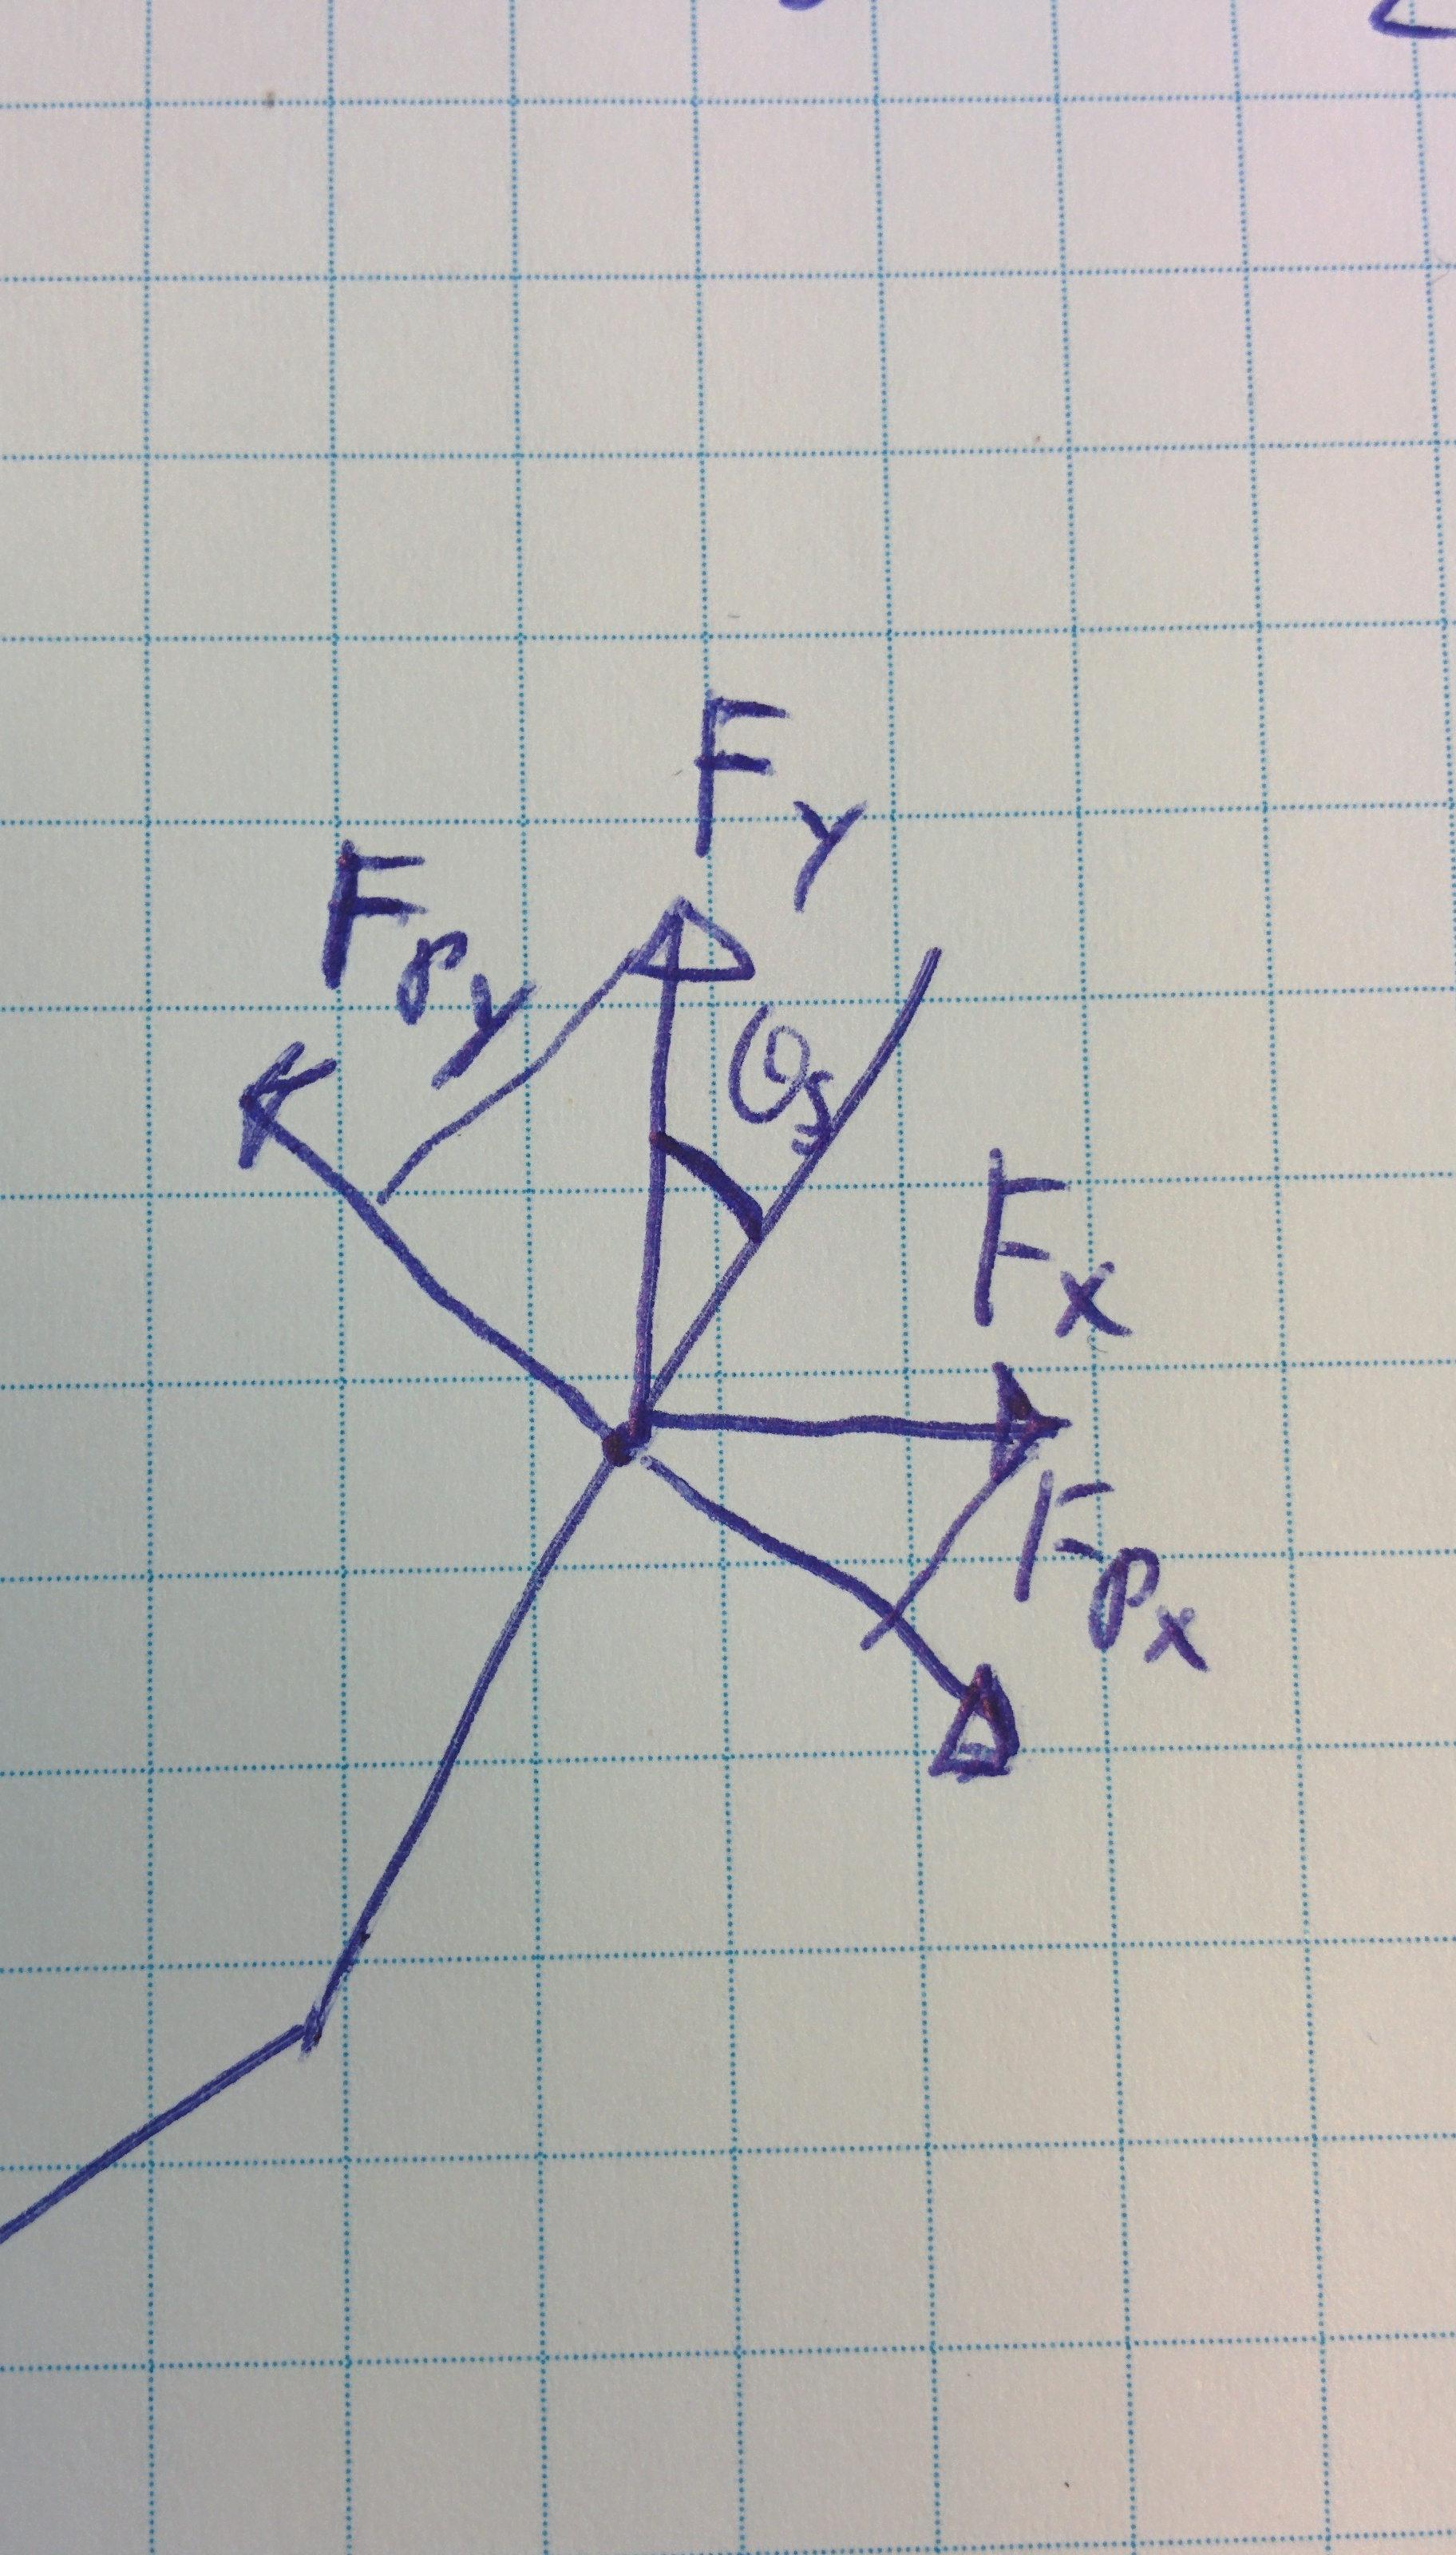
\includegraphics[width=0.25\textwidth]{ForcePerp}
	%		%\caption{Diagram of the forces, $F_x$ and $F_y$, decomposed into perpendicular forces.}
	%		%\label{fig:ForcePerp}
	%		%\end{figure}
	%		
	%		\begin{subequations}\label{eq:perpFxFyRocket}
	%			\begin{flalign}
	%				& F_{px}=F_x\cos(\theta_b) \\
	%				& F_{py}=F_y\sin(\theta_b)  \\
	%				& F_p = F_{px}+F_{py} 
	%			\end{flalign}
	%		\end{subequations}
	%		
	%		The rotary force of the rocket is described by \vref{eq:JrLongRocket}.
	%		\begin{subequations}
	%			\begin{flalign}
	%				J_r\ddot{\theta}_b &=C_g\left(F_x\cos(\theta_b)+F_y\sin(\theta_b)\right)+b_{tb}\dot{\theta}_{tb}  \\
	%				J_r\ddot{\theta}_b = C_g \cdot M_b \Big( &-l_t\ddot{\theta}_t\left(\cos(\theta_t)\cos(\theta_b)+\sin(\theta_t)\sin(\theta_b)\right) \notag \\
	%				& +l_t\dot{\theta}_t^2\left(\sin(\theta_t)\cos(\theta_b)-\cos(\theta_t)\sin(\theta_b)\right) \notag \\
	%				& -C_g\ddot{\theta}_b\left(\cos(\theta_b)\cos(\theta_b)+\sin(\theta_b)\sin(\theta_b)\right) \notag \\
	%				& +C_g\dot{\theta}_b^2\left(\sin(\theta_b)\cos(\theta_b)-\cos(\theta_b)\sin(\theta_b)\right)  \notag \Big)+b_{tb}\dot{\theta}_{tb} \label{eq:JrLongRocket}
	%			\end{flalign}
	%		\end{subequations}
	%		\startexplain
	%			\explain{$b_{tb}$ is the friction created by the ambiant air}{\si{\newton\per\meter}}
	%			\explain{$J_r$ is the torque applied on the rocket}{\si{\newton\per\meter}}
	%		\stopexplain
	%		
	%		Using the trigonometric properties in \vref{eq:trigprop}, \autoref{eq:JrLongRocket} is reduced to \vref{eq:JrShortRocket}.
	%		\begin{subequations} \label{eq:trigprop}
	%			\begin{flalign}
	%				& \cos(\theta_t)\cos(\theta_b)\pm \sin(\theta_t)\sin(\theta_b)=\cos(\theta_t \mp \theta_b)  \\
	%				& \sin(\theta_t)\cos(\theta_b)\pm \cos(\theta_t)\sin(\theta_b) = \sin(\theta_t \pm \theta_b) \\ 
	%				& \cos(\theta_b)^2+\sin(\theta_b)^2=1 
	%			\end{flalign}
	%		\end{subequations}
	%		\begin{flalign}
	%			J_r\ddot{\theta}_b = C_gM_b \Big( &-l_t\ddot{\theta}_t \cos(\theta_t-\theta_b)+l_t\dot{\theta}_t^2 \sin(\theta_t-\theta_b) \notag \\
	%			&-C_g\ddot{\theta}_b \Big)+b_{tb}\dot{\theta}_{tb} \label{eq:JrShortRocket}
	%		\end{flalign}
	%		
	%		This is the nonlinear mathematical model for the system. This will be linearized in order to perform a Laplace transformation. The linearization is made with a 1st order Taylor approximation. The linearization is done at the equilibrium point where the arm is in an upright position i.e. $\theta_b=0$. In the equilibrium point the derivatives of all the inputs and outputs are 0. In this case the inputs and outputs are $\theta_t$ and $\theta_b$ and the operating point is $\bar{\theta}_t=0$ and $\bar{\theta}_b=0$. The nonlinear model is expressed as a function of the inputs and outputs as seen in \vref{eq:nonLinearModelRocket}.
	%		\begin{flalign}\label{eq:nonLinearModelRocket}
	%			f\left(\theta_t, \dot{\theta}_t, \ddot{\theta}_t, \theta_b, \ddot{\theta}_b\right)=C_gM_b \Big( &-l_t\ddot{\theta}_t \cos(\theta_t-\theta_b)+l_t\dot{\theta}_t^2 \sin(\theta_t-\theta_b) \notag \\
	%			&-C_g\ddot{\theta}_b \Big)+b_{tb}\dot{\theta}_{tb}-J_r\ddot{\theta}_b
	%		\end{flalign}
	%		
	%		Generally all equilibriums can be found by setting \vref{eq:nonLinearModelRocket} equal to 0 and the derivatives to 0, and solving for $\theta_t=\bar{\theta}_t$ and $\theta_b=\bar{\theta}_b$. For the rocket the only two equilibriums are the rocket body pointing straight up and straight down. In this project only the postion with the nose pointing straight up is relevent. 
	%		
	%		The 1st order Taylor approximation of an equation with multiple variables is seen in \vref{eq:1stTaylor}.
	%		\begin{flalign}
	%			f\left(\theta_t, \dot{\theta}_t, \ddot{\theta}_t, \theta_b, \ddot{\theta}_b\right) & \approx f\left(\bar{\theta}_t, 0, 0, \bar{\theta}_b, 0\right) + \left. \frac{\partial f}{\partial \theta_t}\right|_{(\bar{\theta}_t, \bar{\theta}_b)} \hat{\theta}_t \notag \\
	%			& \phantom{=} + \left. \frac{\partial f}{\partial \dot{\theta}_t}\right|_{(\bar{\theta}_t, \bar{\theta}_b)} \hat{\dot{\theta}}_t + \left. \frac{\partial f}{\partial \ddot{\theta}_t}\right|_{(\bar{\theta}_t, \bar{\theta}_b)} \hat{\ddot{\theta}}_t \notag \\
	%			& \phantom{=} + \left. \frac{\partial f}{\partial \theta_b}\right|_{(\bar{\theta}_t, \bar{\theta}_b)} \hat{\theta}_b + \left. \frac{\partial f}{\partial \ddot{\theta}_b}\right|_{(\bar{\theta}_t, \bar{\theta}_b)} \hat{\ddot{\theta}}_b \label{eq:1stTaylor}
	%		\end{flalign}
	%		\startexplain
	%		\explain{$\bar{\theta}$ denotes the angle in an operating point}{\si{\radian}}
	%		\explain{$\hat{\theta}$ denotes the angle of the small signal variances}{\si{\radian}}
	%		\stopexplain
	%		
	%		The three terms with sin or cos in \vref{eq:JrShortRocket} will be approximated individually using \vref{eq:1stTaylor}, remembering that $\bar{\theta}=\bar{\dot{\theta}}=\bar{\ddot{\theta}}=0$ in the equilibrium state.
	%		\begin{subequations}
	%			\begin{flalign}
	%				-l_t\ddot{\theta}_t\cos\left(\theta_t-\theta_b\right)  \approx & \ 0 + l_t\bar{\ddot{\theta}}_t\sin\left(\bar{\theta}_t-\bar{\theta}_b\right)\hat{\theta}_t  \notag \\ 
	%				& -l_t\cos\left(\bar{\theta}_t-\bar{\theta}_b\right)\hat{\ddot{\theta}}_t - l_t\bar{\ddot{\theta}}_t\sin\left(\bar{\theta}_t-\bar{\theta}_b\right)\hat{\theta}_b   \\
	%				-l_t\ddot{\theta}_t\cos\left(\theta_t-\theta_b\right) \approx &-l_t\hat{\ddot{\theta}}_t 
	%			\end{flalign} %\bar{\ddot{\theta}}_b
	%		\end{subequations}
	%		\begin{subequations}
	%			\begin{flalign}
	%				l_t\dot{\theta}_t^2\sin\left(\theta_t-\theta_b\right)  \approx &\ 0 + l_t\bar{\dot{\theta}}_t^2\cos\left(\bar{\theta}_t-\bar{\theta}_b\right)\hat{\theta}_t  \notag \\
	%				& + 2l_t\bar{\dot{\theta}}_t\sin\left(\bar{\theta}_t-\bar{\theta}_b\right)\hat{\dot{\theta}}_t-l_t\bar{\dot{\theta}}_t^2\cos\left(\bar{\theta}_t-\bar{\theta}_b\right)\hat{\theta}_b   \\
	%				l_t\dot{\theta}_t^2\sin\left(\bar{\theta}_t-\bar{\theta}_b\right) \approx & \ 0 
	%			\end{flalign}
	%		\end{subequations}
	%		
	%		Inserting the linearized terms in \vref{eq:JrShortRocket} and using the moment of inertia for a rotating stick, $J_r=\frac{1}{12}M_sC_s^2$, the linearized model becomes \eqref{eq:JrFinalRocket}.
	%		\begin{subequations}
	%			\begin{flalign}
	%				& \frac{1}{12}M_bC_g^2\hat{\ddot{\theta}}_b=C_g M_b\left(-l_t\hat{\ddot{\theta}}_t-C_g\hat{\ddot{\theta}}_b\right)+b_{tb}\hat{\dot{\theta}}_{tb}   \\
	%				& \frac{1}{12}M_bC_g^2\hat{\ddot{\theta}}_b+M_bC_g^2\hat{\ddot{\theta}}_b=C_gM_b\left(-l_t\hat{\ddot{\theta}}_t\right)+b_{tb}\hat{\dot{\theta}}_{tb}   \\
	%				& \frac{13}{12}M_bC_g^2\hat{\ddot{\theta}}_b=C_gM_b\left(-l_t\hat{\ddot{\theta}}_t\right)+b_{tb}\hat{\dot{\theta}}_{tb}  \label{eq:TauSmLin} \\
	%				& \hat{\ddot{\theta}}_b=\frac{12}{13C_g}\left(-l_t\hat{\ddot{\theta}}_t\right)+\frac{12b_{tb}\left(\hat{\dot{\theta}}_b-\hat{\dot{\theta}}_t\right)}{13M_bC_g^2} \label{eq:JrFinalRocket}
	%			\end{flalign}
	%		\end{subequations}
	%		
	%		The linearized model is now Laplace transformed in \vref{eq:tfThrusterRocket} in order to find the transfer function.
	%		\begin{subequations}
	%			\begin{flalign}
	%				& s^2\Theta_b=\frac{12}{13C_g}\left(-s^2l_t\Theta_t\right)+s\frac{12b_{tb}}{13M_bC_g^2}\Theta_b-s\frac{12b_{tb}}{13M_bC_g^2}\Theta_t  \\
	%				& \Theta_b\left(s^2-\frac{12b_{tb}}{13M_bC_g^2}s\right)=\Theta_t\left(-\frac{12l_t}{13C_g}s^2-\frac{12b_{tb}}{13M_bC_g^2}s\right)  \\
	%				& \frac{\Theta_b}{\Theta_t}=-\frac{\frac{12l_t}{13C_g}s^2+\frac{12b_{tb}}{13M_bC_g^2}s}{s^2-\frac{12b_{tb}}{13M_bC_g^2}s} \label{eq:tfThrusterRocket}
	%			\end{flalign}
	%		\end{subequations}
	%		
	%		A linearized model in the Laplace domain for the thruster and the rocket body has been derived.
	%
	

